\documentclass{article}
\usepackage{ucs}
\usepackage[T2A]{fontenc}
\usepackage[utf8x]{inputenc}
\usepackage[russian, english]{babel}
\usepackage{listings}
\usepackage{graphicx}
\author{Гвоздев П.А.}
\title{Отчёт по графикам}
\date{23 Мая 2023}



\usepackage{xcolor}

%New colors defined below
\definecolor{codegreen}{rgb}{0,0.6,0}
\definecolor{codegray}{rgb}{0.5,0.5,0.5}
\definecolor{codepurple}{rgb}{0.58,0,0.82}
\definecolor{backcolour}{rgb}{0.95,0.95,0.92}
\lstdefinestyle{mystyle}{
  backgroundcolor=\color{backcolour}, commentstyle=\color{codegreen},
  keywordstyle=\color{magenta},
  numberstyle=\tiny\color{codegray},
  stringstyle=\color{codepurple},
  basicstyle=\ttfamily\footnotesize,
  breakatwhitespace=false,         
  breaklines=true,                 
  captionpos=b,                    
  keepspaces=true,                 
  numbers=left,                    
  numbersep=5pt,                  
  showspaces=false,                
  showstringspaces=false,
  showtabs=false,                  
  tabsize=2
  }
  \lstset{style=mystyle}


\begin{document}
\maketitle

\newpage
\begin{section}{Задача}\\

Вычислить площадь фигуры, которая расположена на плоскости $Oxy.\: 
\\D: y=\arctan(x), y=\arctan(2x-4), y=0$.\\

\begin{lstlisting}[language=Python]
plt.figure(figsize=(5,5))
x=np.linspace(-10,10,1000)
y=np.arctan(x)
y1=np.arctan(2*x-4)

area=np.linspace(0,4,1000)
y_area_top=np.arctan(area)
y_area_low=np.arctan(2*area-4)
plt.fill_between(area,y_area_top,y_area_low,color='orange')

plt.plot(x,y,color='red',lw=2, ls='solid',label=r'$y=\arctan(x)$')
plt.plot(x,y1,lw=2,label=r'$y=\arctan(2x-4)$',color='blue')

plt.text(1.1,0.3,"D", fontsize=12)
plt.xlim(0,5)
plt.grid()
plt.legend(loc=0, prop={'size':12})
plt.title('1')
plt.xlabel('x')
plt.ylabel('y')
\end{lstlisting}


\end{section}

\\
   

\includegraphics[width=0.8\linewidth]{graphic1.png}

%\caption{Иллюстрация к следствию 2}





\newpage
\begin{section}{Задача}\\

Фигура, расположенная вплоскости $Oxy$, вращается около координатной оси.
Вычислить объём полученного тела вращения. \\
$D:\: x=\sqrt{6-y},\: y \geq 2;\: x=4-\sqrt{2y},\:y \leq 2$.
\\
\begin{lstlisting}[language=Python]
plt.figure(figsize=(5,5))
y=np.linspace(2,6,1000)
x=np.sqrt(6-y)
plt.fill_between(x,0,y,color='green')
plt.plot(x,y,color='blue',lw=2,label=r'$x=\sqrt{6-y}, y \geq 2$')
y1=np.linspace(0,2,1000)
x1=4-np.sqrt(2*y1)
plt.plot(x1,y1,color='red',lw=2,label=r'$x=4-\sqrt{2y}, y \leq 2$')
plt.fill_between(x1,0,y1,color='green')


plt.text(1.2,2.2,"D", fontsize=12)
plt.xlim(0,5)
plt.grid()
plt.title('2')
plt.xlabel('x')
plt.ylabel('y')
plt.legend(loc=1, prop={'size':12})
\end{lstlisting}


\end{section}

\\
\includegraphics[width=0.8\linewidth]{graphic2.png}

%\caption{Иллюстрация к следствию 2}





\newpage
\begin{section}{Задача}\\

Вычислить площадь фигуры. Внутри кардиоиды $r=1-\cos(\varphi)$ и одновременно внутри окружности $r=3\cos(\varphi)$.
\\
\begin{lstlisting}[language=Python]
plt.figure(figsize=(5,5))
fi=np.linspace(0,2*np.pi,1000)
r=1+np.cos(fi)
plt.polar(fi,r,color='red',label=r'$r=1-\cos(\varphi)$',lw=2)
r1=3*np.cos(fi)
plt.polar(fi,r1,color='blue',label=r'$r=3\cos(\varphi)$',lw=2)
fi_circle=np.linspace(np.pi/3,5*np.pi/3,1000)
r_circle=3*np.cos(fi_circle)
plt.fill_between(fi_circle,0,r_circle,color='orange')
fi_cardioid=np.linspace(-np.pi/3,np.pi/3,1000)
r_cardioid=1+np.cos(fi_cardioid)
plt.fill_between(fi_cardioid,0,r_cardioid,color='orange')


plt.text(0,1,"D", fontsize=12)
plt.title('3')
plt.ylim(bottom=0)
plt.legend(loc=2, prop={'size':12})
ax = plt.gca()
ax.set_rgrids([i for i in range(4)])
ax.set_rlabel_position(210)
\end{lstlisting}


\end{section}

\\
\includegraphics[width=0.8\linewidth]{graphic3.png}




\newpage
\begin{section}{Задача}\\

Вычислить длину дуги кривой $y=\frac{x^2}{8}-\ln(x)$. 
\\
\begin{lstlisting}[language=Python]
plt.figure(figsize=(5,5))
x=np.linspace(1,2,1000)
y=x*x/8-np.log(x)
plt.plot(x,y,lw=2,color='red',label=r'$y=\frac{x^2}{8}-\ln(x)$')


formatter = ticker.ScalarFormatter(useMathText=True)
formatter.set_scientific(True) 
formatter.set_powerlimits((0,10)) 
ax.yaxis.set_major_formatter(formatter) 

ax=plt.gca()
ax.yaxis.set_major_formatter(formatter)

plt.legend(prop={'size':12})
plt.grid()
plt.title('4')
plt.xlabel('x')
plt.ylabel('y')

\end{lstlisting}


\end{section}

\\
\includegraphics[width=0.8\linewidth]{graphic4.png}





\newpage
\begin{section}{Задача}\\

Вычислить площадь поверхности, полученной при вращении
окружности $x^2+(y-4)^2=1$ вокруг оси $OX$.
\\
\begin{lstlisting}[language=Python]
plt.figure(figsize=(5,5))



x=np.linspace(-1,1,1000)
y=4+np.sqrt(1-np.square(x))
plt.plot(x,y,color='red',lw=2,label=r'$x^2+(y-4)^2=1$')
y1=4-np.sqrt(1-np.square(x))
plt.plot(x,y1,color='red',lw=2)
plt.fill_between(x,y1,y,color='yellow')


plt.text(0,4,"D", fontsize=12)
plt.legend(loc=3, prop={'size':12})
plt.grid()
plt.title('5')
plt.xlabel('x')
plt.ylabel('y')
plt.xlim(-3,3)
plt.ylim(0,6)

\end{lstlisting}


\end{section}

\\
\includegraphics[width=0.8\linewidth]{graphic5.png}




\newpage
\begin{section}{Задача}\\

Исследовать несобственный интеграл на сходимость.\\ \\
$\int_{0}^{+\infty}\frac{1-\cos(x^2+x)}{\sqrt{x^5}}\,dx$
\\
\begin{lstlisting}[language=Python]
plt.figure(figsize=(5,5))

x=np.linspace(0.01,10,1000)
y=(1-np.cos(x*x+x))/np.sqrt(x**5)
plt.plot(x,y,color="red",lw=2,label=r'$y=\frac{1-\cos(x^2+x)}{\sqrt{x^5}}$')
x1=np.linspace(0.2,10,1000)
y1=1/x1
plt.plot(x1,y1,color="blue",lw=2,label=r'$y=\frac{1}{x}}$')


plt.legend(prop ={ 'size' :12})
plt.grid()
plt.title('6')
plt.xlabel('x')
plt.ylabel('y')

plt.show()
\end{lstlisting}


\end{section}

\\
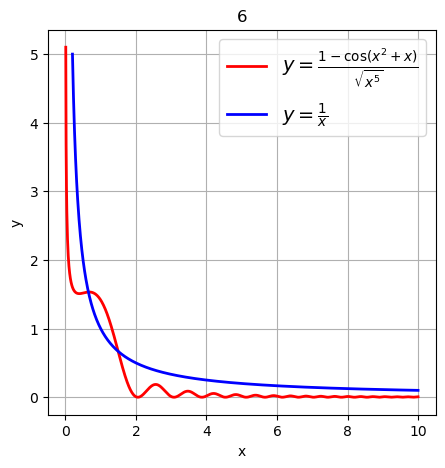
\includegraphics[width=0.8\linewidth]{graphic6.png}



\end{document}